\chapter{Pin Map: Sample Controller - MCU} \label{App:PinMap_MCU_FPGA}
The specific connections between the MCU (STM32 Nucleo F446RE) and Sample Controller (CMOD A7 Artix-7 35T FPGA) can be seen in this appendix. A block diagram with the specific
connections can also be found. Table \ref{tab:App_MCU_FPGA_PinMap} shows all connections between the MCU and Sample Controller. MCU I.Pin refers to MCU Interface Pin, this is the
pin-number assinged to the connection in the Interface of the MCU, see section \ref{subsec:MainProcessorInterface}. The same is true for FPGA I.Pin, refering to FPGA Interface Pin,
see section \ref{subsec:SampleControlInterface}. A diagram of the connections can be seen in figure \ref{fig_App_MCU_FPGA_PinMap}.

\begin{table}[H]
    \begin{tabular}{|m{5.2em}|m{5.2em}|m{6.7em}|m{6.7em}|m{8.7em}|}
    \hline
    \textbf{MCU I.Pin} &   \textbf{FPGA I.Pin} & \textbf{F446RE Pin} & \textbf{Artix 7 Pin} & \textbf{Reference}  \\ \hline
    0 & 0 & CN7-34/PB0 & GPIO45/U7 & DATA bus 0 \\ \hline
    1 & 1 & CN10-24/PB1 & GPIO44/U3 & DATA bus 1 \\ \hline
    2 & 2 & CN10-22/PB2 & GPIO43/W6 & DATA bus 2 \\ \hline
    3 & 3 & CN10-31/PB3 & GPIO42/U2 & DATA bus 3 \\ \hline
    4 & 4 & CN10-27/PB4 & GPIO41/U5 & DATA bus 4 \\ \hline
    5 & 5 & CN10-29/PB5 & GPIO40/W4 & DATA bus 5 \\ \hline
    6 & 6 & CN10-17/PB6 & GPIO39/V5 & DATA bus 6 \\ \hline
    7 & 7 & CN7-21/PB7 & GPIO38/U4 & DATA bus 7 \\ \hline
    8 & 8 & CN7-38/PC0 & GPIO37/V4 & DATA bus 8 \\ \hline
    9 & 9 & CN7-36/PC1 & GPIO36/W5 & DATA bus 9 \\ \hline
    10 & 10 & CN7-35/PC2 & GPIO35/V3 & DATA bus 10 \\ \hline
    11 & 11 & CN7-37/PC3 & GPIO34/W3 & DATA bus 11 \\ \hline
    12 & 12 & CN10-34/PC4 & GPIO33/V2 & DATA bus 12 \\ \hline
    13 & 13 & CN10-6/PC5 & GPIO32/W2 & DATA bus 13 \\ \hline
    14 & 14 & CN10-4/PC6 & GPIO31/U1 & DATA bus 14 \\ \hline
    15 & 15 & CN10-19/PC7 & GPIO30/T2 & DATA bus 15 \\ \hline
    16 & 16 & CN10-1/PC9 & GPIO47/U8 &  Bus CLK\\ \hline
    17 & 17 & CN10-5/PB9 & GPIO46/W7 & R/$\overline{W}^1$ \\ \hline
    18 & 18 & CN10-2/PC8 & GPIO48/V8 & Bus IX  \\ \hline
    \end{tabular}
    \caption*{
        \raggedright
        $\mathbf{^1}$ $\overline{W}$ is active low. When low the MCU will put data on the BUS.\\
      }
    \caption{Pin map of the interconnections between the MCU and the Sample Controller (FPGA).}
    \label{tab:App_MCU_FPGA_PinMap}
  \end{table}


  
\begin{figure}[H]
    \centering
    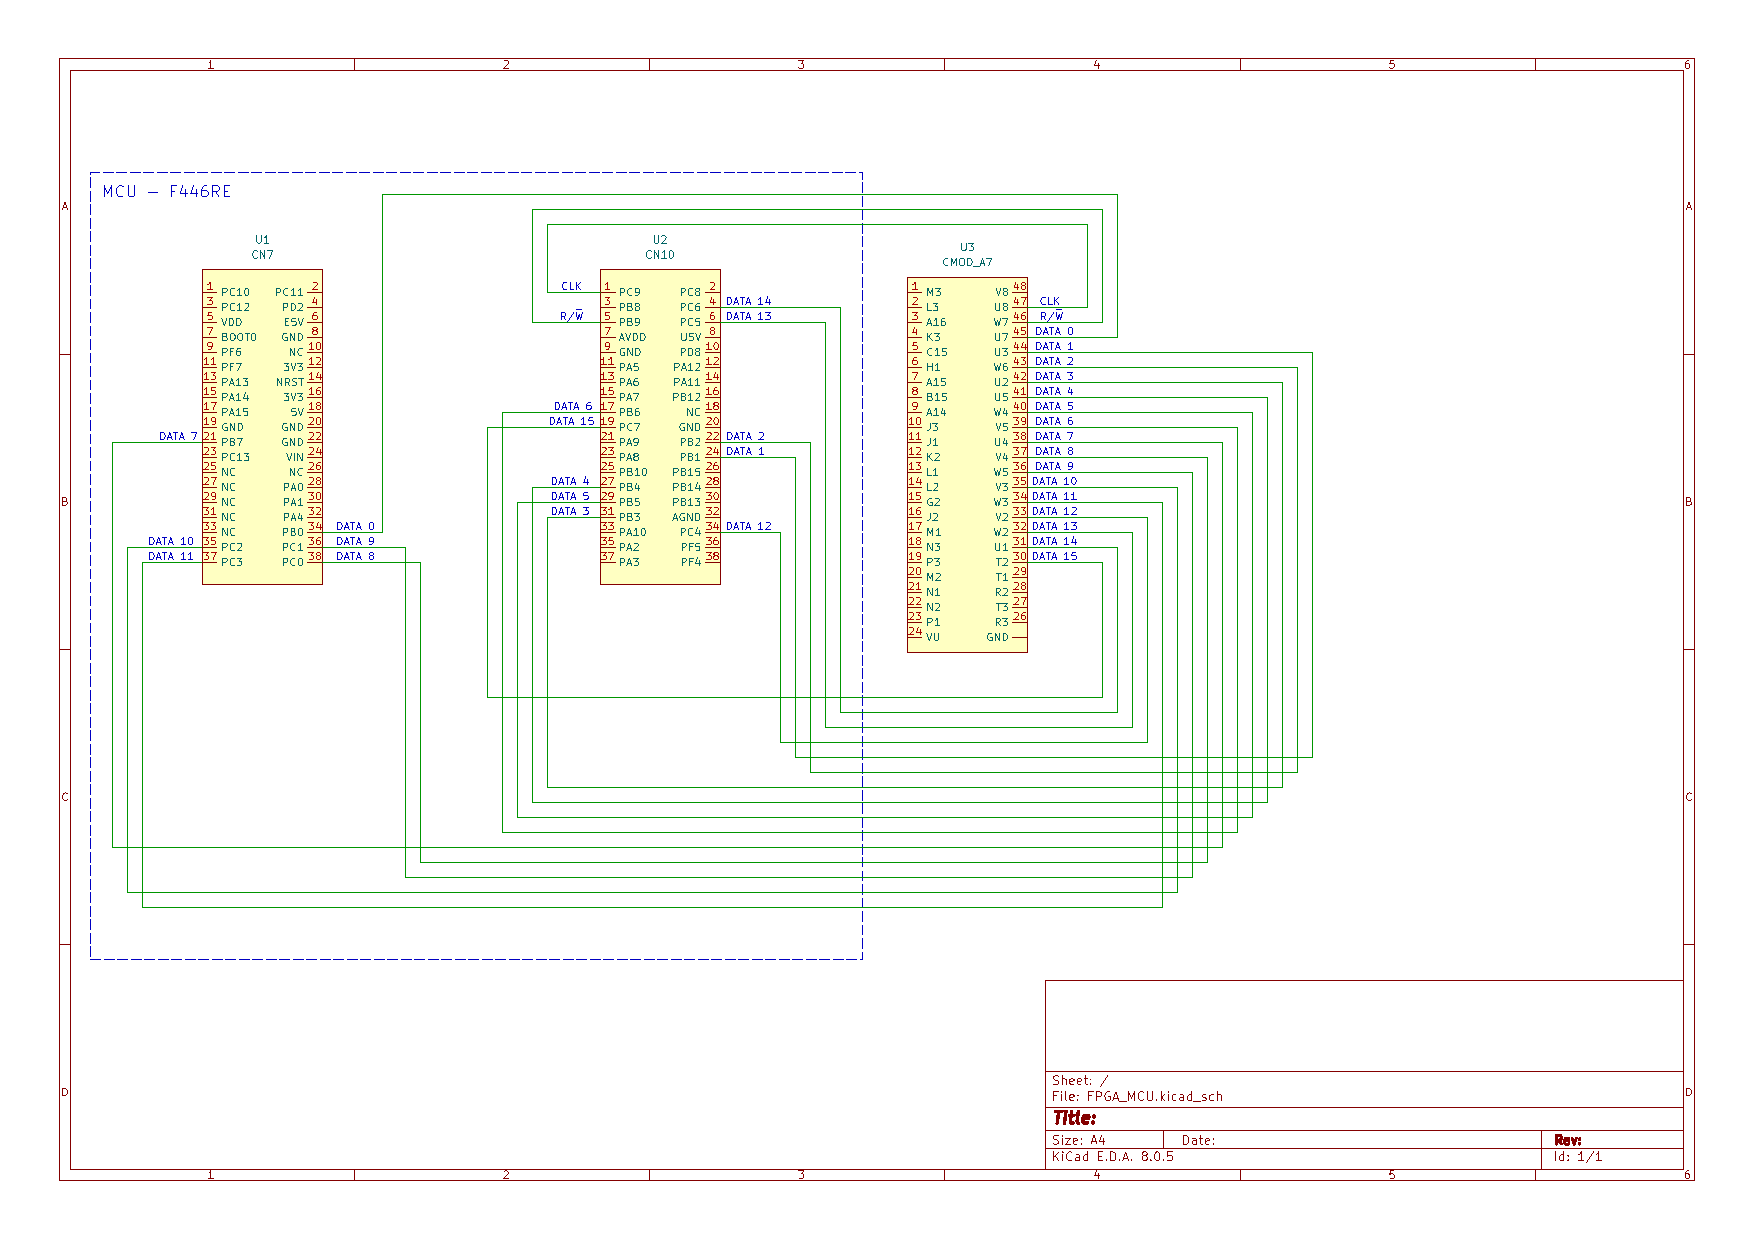
\includegraphics[clip, trim=40 130 190 40,width=1.0\textwidth]{Appendix/Figures/FPGA_MCU_PinOut.pdf}
    \caption{Map of the connections between MCU and Sample Controller (FPGA).}
    \label{fig_App_MCU_FPGA_PinMap}
\end{figure}

